\chapter{Impuse Responses}

\begin{theorem}
    [Linear Time Invariant (LTI) Systems]
    An LTI system is a system that is both linear and time-invariant.
    $$x[n] \rightarrow \boxed{S_\text{LTI}} \rightarrow y[n] = ?$$
\end{theorem}

\section{Special Cases of $x[n]$ (Input Signal)}

\begin{definition}
    [Impulse Response]
    The impulse response of an LTI system is the output of the system when the input is an impulse.
    $$x[n] = \delta[n] \rightarrow \boxed{S_\text{LTI}} \rightarrow h[n]$$
\end{definition}

\begin{figure}
    \centering
    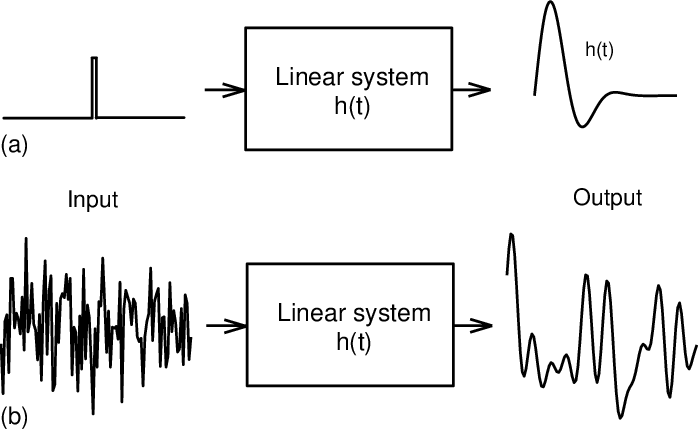
\includegraphics{LECTURE_11/LTI.png}
\end{figure}

\begin{definition}
    [Scaled Impulse Response]
    $$ x[n] = A\delta [n] \rightarrow \boxed{S_\text{LTI}} \rightarrow Ah[n]$$
    $A \in \mathbb{C}$
\end{definition}

\begin{definition}
    [Step Response]
    $$x[n] = \delta[n-k] \rightarrow \boxed{S_\text{LTI}} \rightarrow h[n-k]$$
\end{definition}

\begin{definition}
    [Generalized Impulse Response]
    $$ \sum_{k\in \mathbb{Z}} x[k] \delta[n-k] \rightarrow \boxed{S_\text{LTI}} \rightarrow y[n] = \sum_{k\in \mathbb{Z}} x[k] h[n-k]$$
\end{definition}


\begin{definition}
    [Convolution]
    Let $x\in \mathbb{C}^{\mathbb{Z}}$ and $h\in \mathbb{C}^{\mathbb{Z}}$ be discrete-time signals.\\
    We define a new signal $y\in \mathbb{C}^{\mathbb{Z}}$ as the convolution of $x$ and $h$. We denote this as $y = x * h$.
    $$ y[n] = (x*h)[n] = \sum_{k\in \mathbb{Z}} x[k] h[n-k]$$
\end{definition}

\begin{example}
    [Convolution in polynomial multiplication]
    \begin{align*}
        a_0 + a_1 x + a_2 x^2 + \ldots + a_n x^n &= (a_0 + a_1 x + a_2 x^2 + \ldots + a_n x^n) & \times \\
    \end{align*}
\end{example}